\documentclass{standalone}
\usepackage{tikz}
\usetikzlibrary{patterns, positioning}
\usepackage[sfdefault]{ClearSans} %% option 'sfdefault' activates Clear Sans as the default text font
\usepackage[T1]{fontenc}

\begin{document}
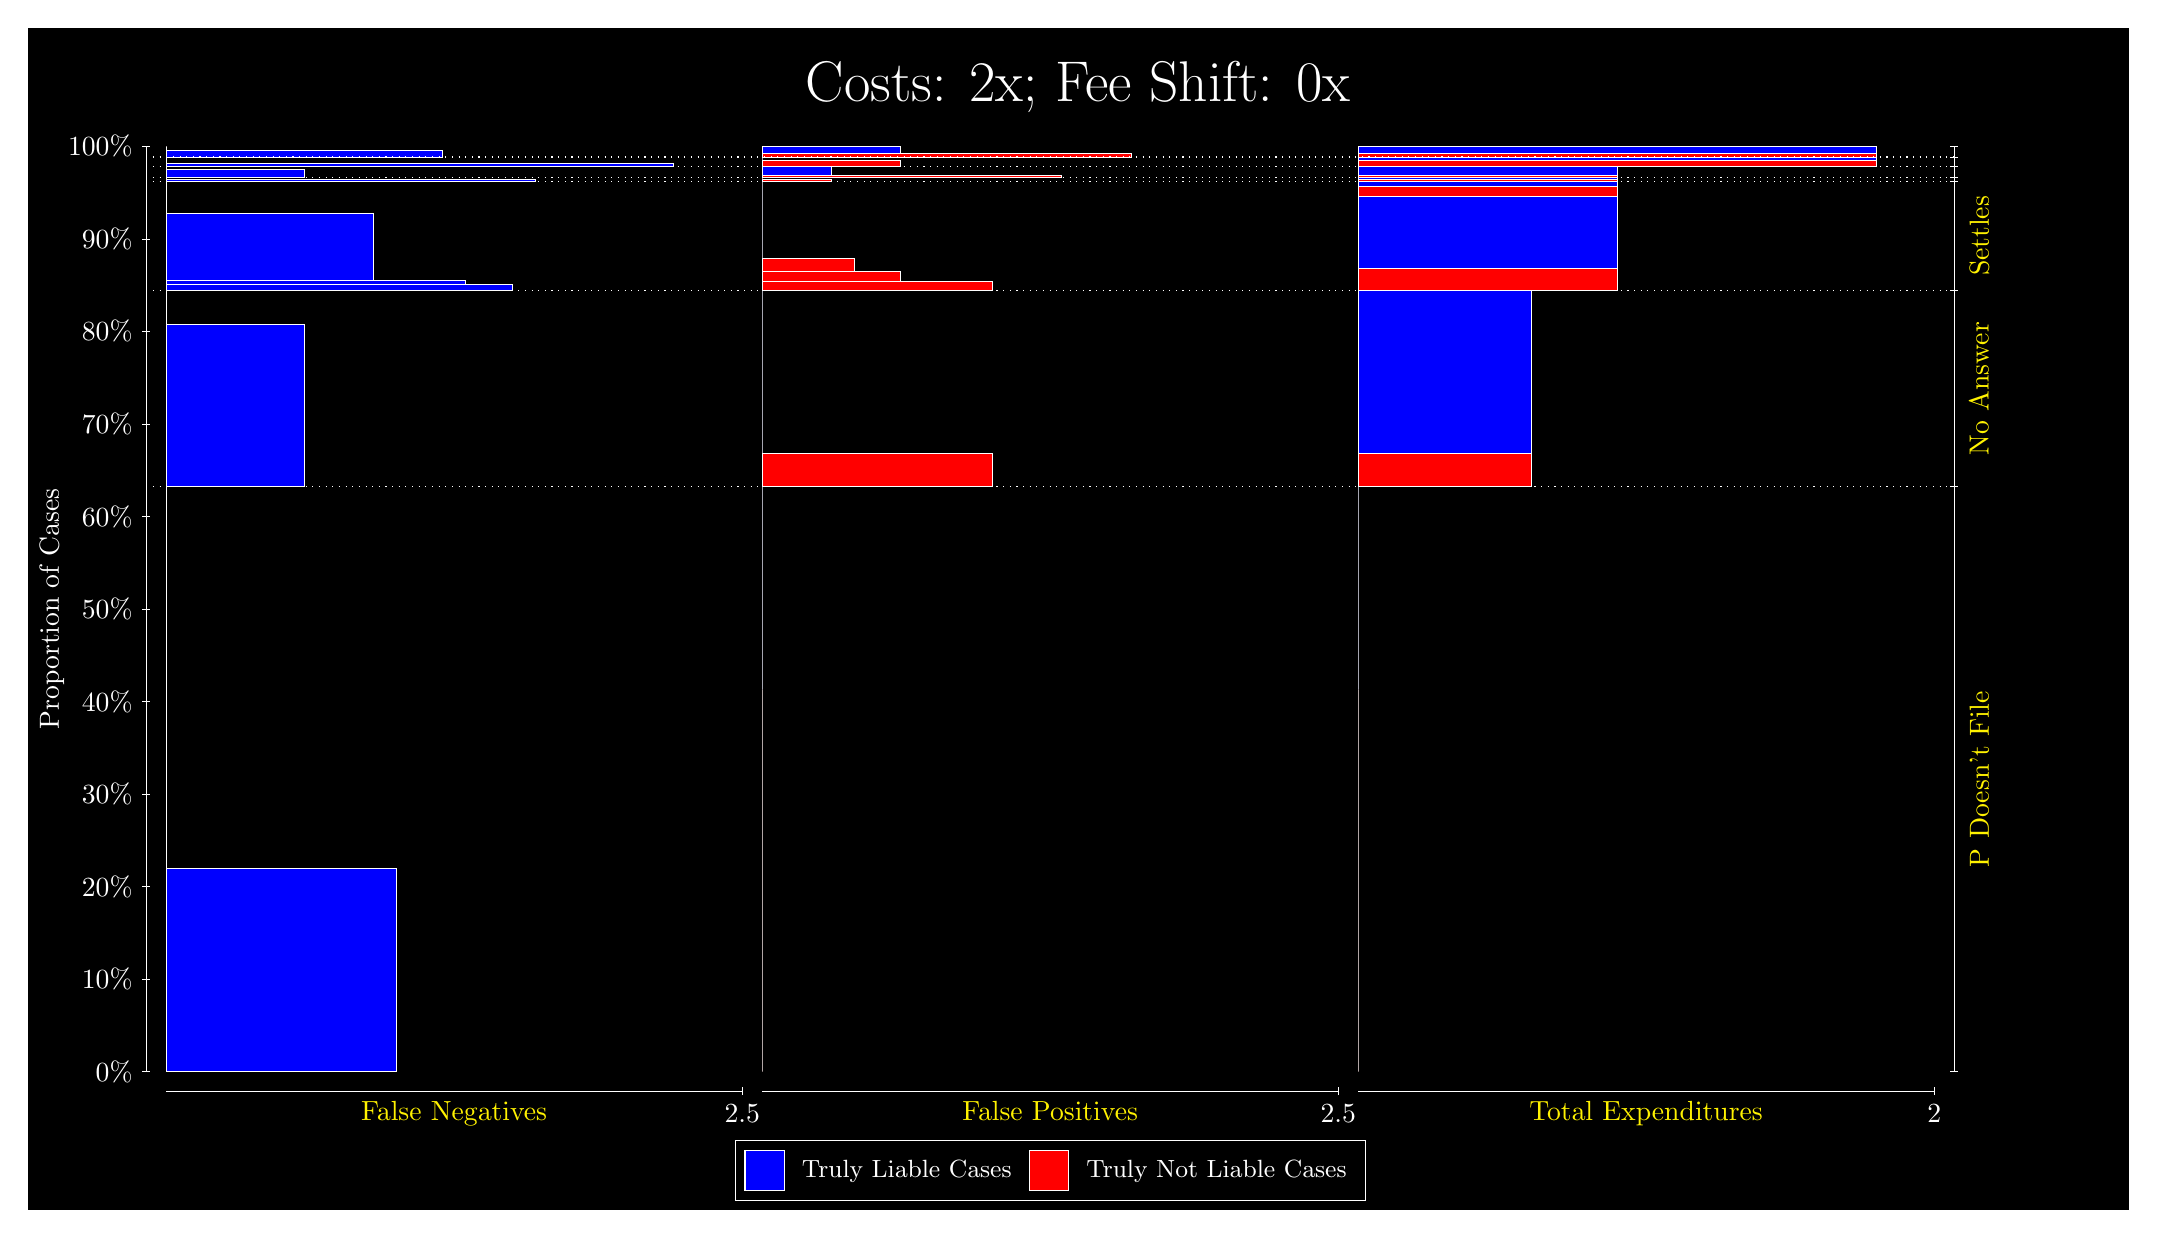
\begin{tikzpicture}
\draw[fill=black] (0,0) rectangle (26.667,15);
\draw[text=white] (0,13.5) rectangle (26.667,15) node[midway] {\huge Costs: 2x; Fee Shift: 0x};
\draw[white, very thin] (1.5,1.75) -- (1.5,13.5);
\node[rotate=90, text=white, anchor=center] at (0.3, 7.625) {Proportion of Cases};
\draw[white, very thin] (1.45,1.75) -- (1.55,1.75);
\node[text=white, anchor=east] at (1.45, 1.75) {0\%};
\draw[white, very thin] (1.45,2.925) -- (1.55,2.925);
\node[text=white, anchor=east] at (1.45, 2.925) {10\%};
\draw[white, very thin] (1.45,4.1) -- (1.55,4.1);
\node[text=white, anchor=east] at (1.45, 4.1) {20\%};
\draw[white, very thin] (1.45,5.275) -- (1.55,5.275);
\node[text=white, anchor=east] at (1.45, 5.275) {30\%};
\draw[white, very thin] (1.45,6.45) -- (1.55,6.45);
\node[text=white, anchor=east] at (1.45, 6.45) {40\%};
\draw[white, very thin] (1.45,7.625) -- (1.55,7.625);
\node[text=white, anchor=east] at (1.45, 7.625) {50\%};
\draw[white, very thin] (1.45,8.8) -- (1.55,8.8);
\node[text=white, anchor=east] at (1.45, 8.8) {60\%};
\draw[white, very thin] (1.45,9.975) -- (1.55,9.975);
\node[text=white, anchor=east] at (1.45, 9.975) {70\%};
\draw[white, very thin] (1.45,11.15) -- (1.55,11.15);
\node[text=white, anchor=east] at (1.45, 11.15) {80\%};
\draw[white, very thin] (1.45,12.325) -- (1.55,12.325);
\node[text=white, anchor=east] at (1.45, 12.325) {90\%};
\draw[white, very thin] (1.45,13.5) -- (1.55,13.5);
\node[text=white, anchor=east] at (1.45, 13.5) {100\%};

\draw[white, very thin] (24.457,1.75) -- (24.457,13.5);
\draw[white, very thin] (24.407,1.75) -- (24.507,1.75);
\node[anchor=west] at (24.407, 1.75) {};
\draw[white, very thin] (24.407,9.1777) -- (24.507,9.1777);
\node[anchor=west] at (24.407, 9.1777) {};
\draw[white, very thin] (24.407,11.668) -- (24.507,11.668);
\node[anchor=west] at (24.407, 11.668) {};
\draw[white, very thin] (24.407,13.057) -- (24.507,13.057);
\node[anchor=west] at (24.407, 13.057) {};
\draw[white, very thin] (24.407,13.101) -- (24.507,13.101);
\node[anchor=west] at (24.407, 13.101) {};
\draw[white, very thin] (24.407,13.243) -- (24.507,13.243);
\node[anchor=west] at (24.407, 13.243) {};
\draw[white, very thin] (24.407,13.365) -- (24.507,13.365);
\node[anchor=west] at (24.407, 13.365) {};
\draw[white, very thin] (24.407,13.5) -- (24.507,13.5);
\node[anchor=west] at (24.407, 13.5) {};

\draw[white, very thin, fill=blue] (1.75,1.75) rectangle (4.6775,4.3256);
\draw[white, very thin, fill=red] (1.75,4.3256) rectangle (1.75,9.1777);
\draw[white, very thin, fill=blue] (1.75,9.1777) rectangle (3.5065,11.239);
\draw[white, very thin, fill=red] (1.75,11.239) rectangle (1.75,11.668);
\draw[white, very thin, fill=blue] (1.75,11.668) rectangle (6.1413,11.742);
\draw[white, very thin, fill=blue] (1.75,11.742) rectangle (5.5558,11.802);
\draw[white, very thin, fill=blue] (1.75,11.802) rectangle (4.3848,12.645);
\draw[white, very thin, fill=red] (1.75,12.645) rectangle (1.75,13.057);
\draw[white, very thin, fill=blue] (1.75,13.057) rectangle (6.4341,13.077);
\draw[white, very thin, fill=red] (1.75,13.077) rectangle (1.75,13.101);
\draw[white, very thin, fill=blue] (1.75,13.101) rectangle (3.5065,13.206);
\draw[white, very thin, fill=red] (1.75,13.206) rectangle (1.75,13.243);
\draw[white, very thin, fill=blue] (1.75,13.243) rectangle (8.1906,13.288);
\draw[white, very thin, fill=red] (1.75,13.288) rectangle (1.75,13.365);
\draw[white, very thin, fill=blue] (1.75,13.365) rectangle (5.2631,13.455);
\draw[white, very thin, fill=red] (1.75,13.455) rectangle (1.75,13.5);
\draw[white, very thin, fill=red] (9.3189,1.75) rectangle (9.3189,6.6021);
\draw[white, very thin, fill=blue] (9.3189,6.6021) rectangle (9.3189,9.1777);
\draw[white, very thin, fill=red] (9.3189,9.1777) rectangle (12.246,9.6067);
\draw[white, very thin, fill=blue] (9.3189,9.6067) rectangle (9.3189,11.668);
\draw[white, very thin, fill=red] (9.3189,11.668) rectangle (12.246,11.78);
\draw[white, very thin, fill=red] (9.3189,11.78) rectangle (11.075,11.91);
\draw[white, very thin, fill=red] (9.3189,11.91) rectangle (10.49,12.08);
\draw[white, very thin, fill=blue] (9.3189,12.08) rectangle (9.3189,13.057);
\draw[white, very thin, fill=red] (9.3189,13.057) rectangle (10.197,13.08);
\draw[white, very thin, fill=blue] (9.3189,13.08) rectangle (9.3189,13.101);
\draw[white, very thin, fill=red] (9.3189,13.101) rectangle (13.125,13.138);
\draw[white, very thin, fill=blue] (9.3189,13.138) rectangle (10.197,13.243);
\draw[white, very thin, fill=red] (9.3189,13.243) rectangle (11.075,13.32);
\draw[white, very thin, fill=blue] (9.3189,13.32) rectangle (9.3189,13.365);
\draw[white, very thin, fill=red] (9.3189,13.365) rectangle (14.003,13.41);
\draw[white, very thin, fill=blue] (9.3189,13.41) rectangle (11.075,13.5);
\draw[white, very thin, fill=red] (16.888,1.75) rectangle (16.888,6.6021);
\draw[white, very thin, fill=blue] (16.888,6.6021) rectangle (16.888,9.1777);
\draw[white, very thin, fill=red] (16.888,9.1777) rectangle (19.083,9.6067);
\draw[white, very thin, fill=blue] (16.888,9.6067) rectangle (19.083,11.668);
\draw[white, very thin, fill=red] (16.888,11.668) rectangle (20.181,11.95);
\draw[white, very thin, fill=blue] (16.888,11.95) rectangle (20.181,12.867);
\draw[white, very thin, fill=red] (16.888,12.867) rectangle (20.181,12.997);
\draw[white, very thin, fill=blue] (16.888,12.997) rectangle (20.181,13.057);
\draw[white, very thin, fill=red] (16.888,13.057) rectangle (20.181,13.08);
\draw[white, very thin, fill=blue] (16.888,13.08) rectangle (20.181,13.101);
\draw[white, very thin, fill=red] (16.888,13.101) rectangle (20.181,13.138);
\draw[white, very thin, fill=blue] (16.888,13.138) rectangle (20.181,13.243);
\draw[white, very thin, fill=red] (16.888,13.243) rectangle (23.475,13.32);
\draw[white, very thin, fill=blue] (16.888,13.32) rectangle (23.475,13.365);
\draw[white, very thin, fill=red] (16.888,13.365) rectangle (23.475,13.41);
\draw[white, very thin, fill=blue] (16.888,13.41) rectangle (23.475,13.5);
\draw[white, dotted] (1.5,9.1777) -- (24.457,9.1777);
\draw[white, dotted] (1.5,11.668) -- (24.457,11.668);
\draw[white, dotted] (1.5,13.057) -- (24.457,13.057);
\draw[white, dotted] (1.5,13.101) -- (24.457,13.101);
\draw[white, dotted] (1.5,13.243) -- (24.457,13.243);
\draw[white, dotted] (1.5,13.365) -- (24.457,13.365);
\draw[white, very thin] (1.75,1.5) -- (9.0689,1.5);
\node[text=yellow, anchor=north] at (5.4094, 1.5) {False Negatives};
\draw[white, very thin] (9.0689,1.45) -- (9.0689,1.55);
\node[text=white, anchor=north] at (9.0689, 1.45) {2.5};

\draw[white, very thin] (9.3189,1.5) -- (16.638,1.5);
\node[text=yellow, anchor=north] at (12.978, 1.5) {False Positives};
\draw[white, very thin] (16.638,1.45) -- (16.638,1.55);
\node[text=white, anchor=north] at (16.638, 1.45) {2.5};

\draw[white, very thin] (16.888,1.5) -- (24.207,1.5);
\node[text=yellow, anchor=north] at (20.547, 1.5) {Total Expenditures};
\draw[white, very thin] (24.207,1.45) -- (24.207,1.55);
\node[text=white, anchor=north] at (24.207, 1.45) {2};

\node[text=yellow, centered, rotate=90] at (24.777, 5.4639) {P Doesn't File};
\node[text=yellow, centered, rotate=90] at (24.777, 10.423) {No Answer};
\node[text=yellow, centered, rotate=90] at (24.777, 12.363) {Settles};





\draw (12.978300999999998,1.5) node[draw=none] (baseCoordinate) {};
\begin{scope}[align=center]
        \matrix[scale=0.5, draw=white, below=0.5cm of baseCoordinate, nodes={draw}, column sep=0.1cm]{
            \node[rectangle, draw, minimum width=0.5cm, minimum height=0.5cm, fill=blue] {}; &
            \node[draw=none, font=\small, text=white] (B) {Truly Liable Cases}; &
            \node[rectangle, draw, minimum width=0.5cm, minimum height=0.5cm, fill=red] {}; &
            \node[draw=none, font=\small, text=white] (B) {Truly Not Liable Cases}; \\
            };
\end{scope}

\end{tikzpicture}
\end{document}